% preamble

\documentclass[10pt]{article}
\usepackage[paperwidth=40in, paperheight=40in]{geometry}
\usepackage[usenames]{color} %used for font color
\usepackage{amssymb} %maths
\usepackage{amsmath} %maths
\usepackage[utf8]{inputenc} %useful to type directly diacritic characters

%%% Sans serif text font
\usepackage[scaled]{helvet}
\renewcommand*\familydefault{\sfdefault}\usepackage[T1]{fontenc}
%%%

\usepackage{skull}
\usepackage{tikz}
\usetikzlibrary{positioning}
\usetikzlibrary{arrows}
\usetikzlibrary{fit}
\usetikzlibrary{calc}
\usetikzlibrary{automata}
\usetikzlibrary{decorations.markings}
\usetikzlibrary{decorations.pathreplacing}

\tikzset{>=latex}
\tikzstyle{snode}=[black,draw=black,line width=1.5pt,shape=circle,fill=white,minimum size=8mm]
\tikzstyle{obnode}=[black,draw=black,line width=1.5pt,shape=circle,fill=black!20!white,minimum size=8mm]
\tikzstyle{detnode}=[black,draw=black,line width=1.5pt,densely dotted,shape=circle,fill=white,minimum size=8mm]
\tikzstyle{constnode}=[black,draw=black,line width=1.5pt,shape=rectangle,fill=white,minimum size=8mm]
\tikzstyle{distnode}=[black,draw=black,line width=1.5pt,dotted,shape=rectangle,fill=white,minimum size=8mm]
\tikzstyle{mincnode}=[black,draw=black,line width=0.75pt,shape=rectangle,fill=white,minimum size=3mm]
\tikzstyle{blnode}=[white,draw=black,line width=1pt,shape=circle,fill=black,minimum size=1mm,font=\scriptsize,inner sep=1pt]
\tikzstyle{ylnode}=[black,draw=black,line width=1pt,shape=circle,fill=yellow,minimum size=1mm,font=\scriptsize,inner sep=1pt]
\tikzstyle{aro}=[line width=2pt,color=black]
\tikzstyle{taro}=[->,line width=2pt,color=black]
\tikzstyle{thintaro}=[->,line width=0.75pt,color=black]
\tikzstyle{dtaro}=[->,line width=2pt, dashed,color=black]
\tikzstyle{smod}=[black, draw=black, line width=2pt, fill=white, shape=rectangle, rounded corners, minimum size=10mm, minimum width=20mm]
\tikzstyle{obmod}=[black, draw=black, line width=2pt, fill=black!20!white, shape=rectangle, rounded corners, minimum size=10mm, minimum width=20mm, minimum width=20mm]
\tikzstyle{letter} = [black, font=\bf \Huge]

\tikzset{dot/.style={circle,fill=#1,inner sep=0,minimum size=3pt}}

\begin{document}
\[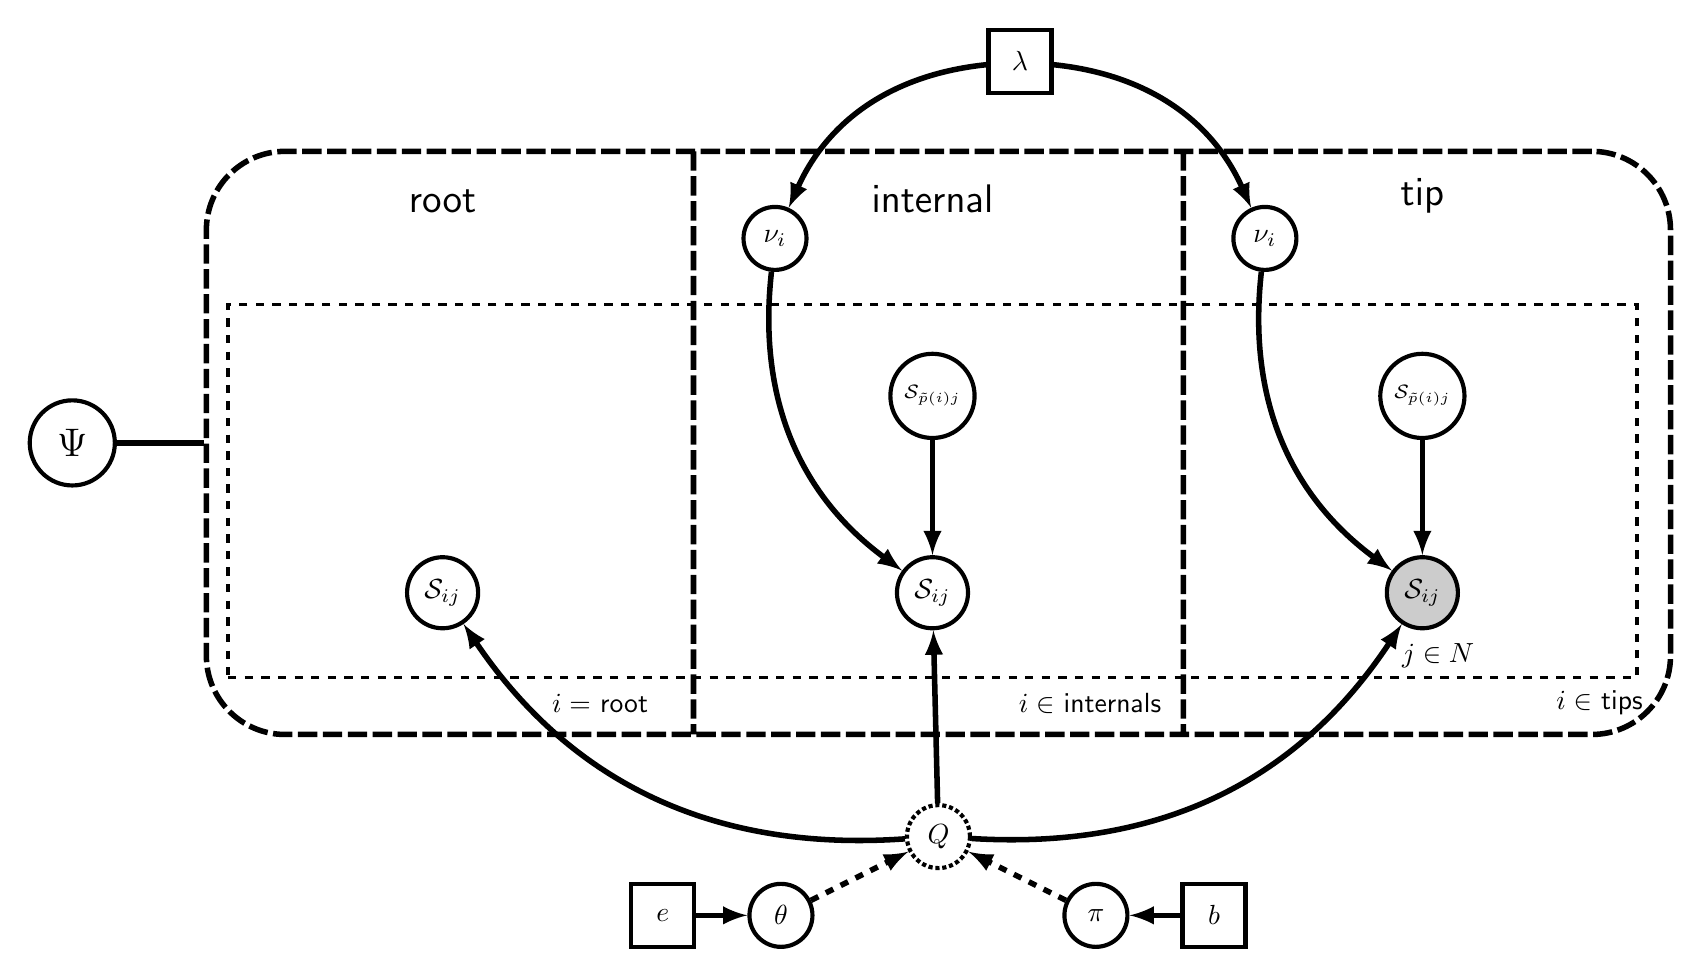
\begin{tikzpicture}
\node[black,draw=black,line width=2pt, dashed,dash pattern=on 7pt off 2pt,shape=rectangle,inner sep=30mm,rounded corners=1cm, rectangle split, rectangle split horizontal, rectangle split parts=3, rectangle split empty part height=9ex] (tp) at (-2,-2.5) { \nodepart {two}  };
\node [font=\Large] at (tp.text) [above=3.5]{root};
\node [font=\Large] at (tp.two) [above=3.5]{internal};
\node [font=\Large] at (tp.three) [above=3.5]{tip};
\node [obnode] (tn) at ($(tp.three)-(0,1.2)$) {$\mathcal{S}_{ij}$};
\node [snode] (in) at ($(tp.two)-(0,1.2)$) {$\mathcal{S}_{ij}$};
\node [snode] (rn) at ($(tp.text)-(0,1.2)$) {$\mathcal{S}_{ij}$};
\node [font=\scriptsize,snode] (pin) at ($(in)+(0,2.5)$) {$\mathcal{S}_{\tilde{p}(i)j}$};
\node [font=\scriptsize,snode] (ptn) at ($(tn)+(0,2.5)$) {$\mathcal{S}_{\tilde{p}(i)j}$};
\draw [taro] (ptn) -- (tn) ;
\draw [taro] (pin) -- (in) ;
\node (a1) at ($(rn)-(2,0)$) { };
\node (a2) at ($(tn)+(2,0)$) { };
\node[rectangle,dashed, very thick, inner sep=6mm, draw=black!100, fit = (tn) (in) (ptn) (a1) (a2)] (siteplate) {};
\node at ($(tn)+(0.2,-0.8)$) {$j \in N$};
\node at ($(tp.text)-(-2.0,2.6)$) {$i =$ root};
\node at ($(tp.two)-(-2.0,2.6)$) {$i \in$ internals};
\node at ($(tp.three)-(-2.25,2.6)$) {$i \in$ tips};
\node [detnode] (qn) at ($(tp)-(0,5)$) {$Q$};
\draw [taro] (qn) -- (in) ;
\draw [taro] (qn) edge[bend right] (tn) ;
\draw [taro] (qn) edge[bend left] (rn) ;
\node [snode] (en) at ($(qn)-(2,1)$) {$\theta$};
\node [snode] (bn) at ($(qn)-(-2,1)$) {$\pi$};
\draw [dtaro] (en) -- (qn) ;
\draw [dtaro] (bn) -- (qn) ;
\node [constnode] (pen) at ($(en)-(1.5,0)$) {$e$};
\node [constnode] (pbn) at ($(bn)-(-1.5,0)$) {$b$};
\draw [taro] (pen) -- (en) ;
\draw [taro] (pbn) -- (bn) ;
\node [snode] (lin) at ($(in)+(-2,4.5)$) {$\nu_i$};
\node [snode] (ltn) at ($(tn)+(-2,4.5)$) {$\nu_i$};
\draw [taro] (lin) edge[bend right](in) ;
\draw [taro] (ltn) edge[bend right](tn) ;
\coordinate (Middle) at ($(lin)!0.5!(ltn)$);
\node [constnode] (lamb) at ($(Middle)+(0,2.25)$) {$\lambda$};
\draw [taro] (lamb) edge[bend left](ltn) ;
\draw [taro] (lamb) edge[bend right](lin) ;
\node[snode,inner sep=2mm] (topo) at ($(tp)+(-11,0)$) {\Large $\Psi$};
\draw[-,line width=2pt] (topo) -- (tp) ;
\end{tikzpicture}



\]
\end{document}